\section{Durchführung}
\label{sec:Durchführung}
Um sowohl die Strahlen- als auch die Wellenoptik genauer zu untersuchen,
stand eine Grundplatte, unter der unterschiedliche Vorlagen mit Winkelskalen
platziert werden konnten. Darauf befestigt waren zwei Laserdioden, eine mit der 
Wellenlänge $\lambda_r = 635 \si{\nano\m}$, also rotem Licht, und eine mit
Wellenlänge $\lambda_g = 532 \si{\nano\m}$, grünem Licht, die im 
Halbkreis bewegt werden konnten.\\
Des weiteren wurden für die unterschiedlichen Versuche verschiedene optische
Elemente (zu sehen in Abbildung \ref{fig:elemente}) im Zentrum des Halbkreises platziert.

\begin{figure}
    \centering
    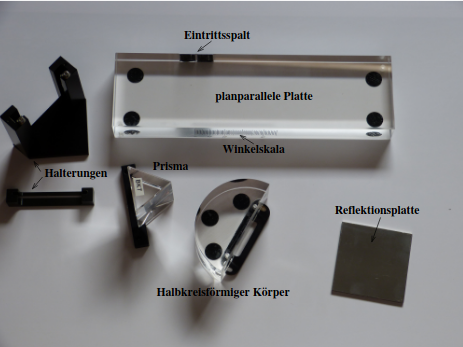
\includegraphics[width=0.75\textwidth]{werkzeug.png}
    \caption{Optische Elemente für verschiedene Untersuchungen.}
    \label{fig:elemente}
\end{figure}

\subsection{Reflexion}
Zunächst wurde ein Spiegel im Zentrum des Halbkreises platziert. Der Versuchsaufbau
ist in Abbildung \ref{fig:aufbau} gezeigt.

\begin{figure}
    \centering
    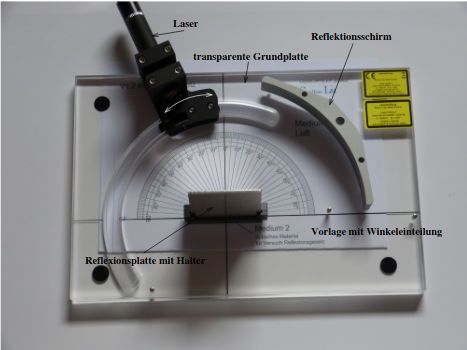
\includegraphics[width=0.75\textwidth]{aufbauuu.png}
    \caption{Versuchsaufbau zur Untersuchung der Reflexion.}
    \label{fig:aufbau}
\end{figure}

Mit dem grünen Laser wurde für 7 Einfallswinkel der Reflexionswinkel gemessen.

\subsection{Brechung}
Um die Brechung im optisch dichteren Medium zu betrachten, wurde eine Plexiglasplatte
mit einer an einer Seite angeklebten Winkelskala,
wie sie in Abbildung \ref{fig:elemente} zu sehen ist, verwendet. Die 
Platte wurde so platziert, dass der Eintrittsspalt zur Winkelskala zeigt.
Auch hier wurden 7 Einfallswinkel betrachtet.

\subsection{Planparallele Platten}
Der Versuch wurde Analog wie der zur Brechung aufgebaut. Zusätzlich wurde
ein Transmissionsschirm aufgestellt. Mit dem grünen Laser wurde 
für 5 Einfallswinkel der 
Strahlversatz gemessen.

\subsection{Prisma}
Zur Betrachtung der Brechung am Prisma wurde im Zentrum des Halbkreises
ein Prisma aus Kronglas platziert. Um die Dispersion zu messen, wurden sowohl 
für den grünen als auch den roten Laser bei 5 Einfallswinkeln die Ablenkung gemessen.

\subsection{Beugung am Gitter}
Zunächst wurde der Versuch ohne Beugungsgitter in der Mitte des Halbkreises aufgebaut.
Dabei traf das Laserlicht den Transmissionsschirm bei einem Winkel von 0 Grad. 
Es wurden für drei Beugungsgitter unterschiedlicher Gitterkonstante
jeweils mit dem roten und dem grünen Laser die 
Maxima gemessen. 